\subsection{Reverb}
\index{Reverb}
In any real sound there will be some amount of \textit{reverb} or \textit{reverberation}, which gives
the sound a spatial character. This is caused by the sound reflecting off the walls and objects of the
environment (room), creating a myriad of indistinguishable.

\begin{figure}[h]
\centering
\begin{subfigure}{0.3\textwidth}
\centering
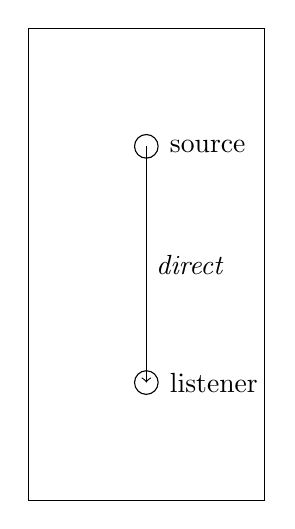
\begin{tikzpicture}[scale=1.5, domain=0:4]
    \draw (0,0) rectangle (2,4);
    \draw [->] (1, 3) -- (1, 1) node [pos=0.5, right, align=left] {\textit{direct}};
    \draw (1, 3) circle [radius=0.1] node [right=5, align=left] {source};
    \draw (1, 1) circle [radius=0.1] node [right=5, align=left] {listener};
\end{tikzpicture}
\end{subfigure}
\begin{subfigure}{0.3\textwidth}
\centering
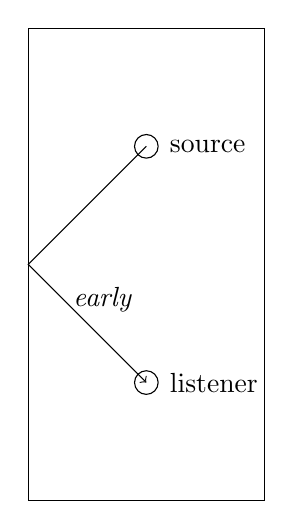
\begin{tikzpicture}[scale=1.5, domain=0:4]
    \draw (0,0) rectangle (2,4);
    \draw [->] (1, 3) -- (0, 2) -- (1, 1) node [pos=0.3, right, align=left] {\textit{early}};
    \draw (1, 3) circle [radius=0.1] node [right=5, align=left] {source};
    \draw (1, 1) circle [radius=0.1] node [right=5, align=left] {listener};
\end{tikzpicture}
\end{subfigure}
\begin{subfigure}{0.3\textwidth}
\centering
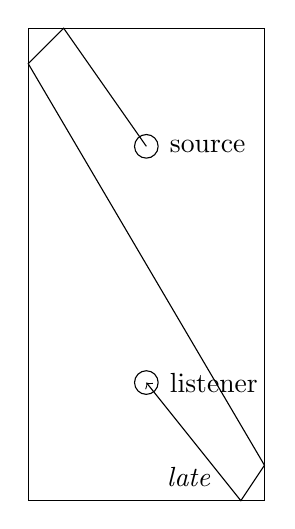
\begin{tikzpicture}[scale=1.5, domain=0:4]
    \draw (0,0) rectangle (2,4);
    \draw [->] (1, 3) -- (0.3, 4) -- (0, 3.7) -- (2, 0.3) -- (1.8, 0) -- (1, 1) node [pos=0.2, left, align=right] {\textit{late}} ;
    \draw (1, 3) circle [radius=0.1] node [right=5, align=left] {source};
    \draw (1, 1) circle [radius=0.1] node [right=5, align=left] {listener};
\end{tikzpicture}
\end{subfigure}
\end{figure}

The character of the reverb is highly dependent on the shape of the room. Irregularities and materials of real rooms makes real-time simulation
unsuitable. Therefore reverb is often modelled via the following three types of reflections:

\begin{description}
    \item[direct reflections] that travel directly from the source to the listener.
    \item[early reflections] where the sound is reflected off close by surfaces.
    \item[late reflections] where the sound is reflected multiple times or off distant surfaces. This is usually very dense with hundreds
        or thousands reflections.
\end{description}

The transmission of sound in air and reflections off the surfaces of the room causes an exponential decay in amplitude. The time it takes for the level to be attenuated $60dB$ is referred to as the \textit{reverberation time}.
\\~\\
\textit{For more information on reverbs, \cite{Gardner:2002} is recommended.}
